\section{Related work}

\subsection{Multilayer perceptron}
The multilayer perceptron is an artificial neural network (ANN) formed by
multiple layers, in such a way that it has the capacity to solve problems that
are not linearly separable, which is the main limitation of the perceptron (also
called simple perceptron).\\

\textbf{Linearly separable:} Linearly separable data is data that can be
separated by a line. To model this concept in a simple way, we are going to use
the logical functions AND and OR (which are linearly separable)
\cite{perceptron}.

\begin{figure}[H]
    \centering
    \begin{subfigure}[b]{0.8\textwidth}
        \centering
        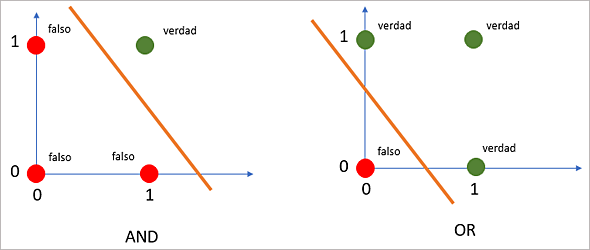
\includegraphics[width=\textwidth]{Figures/2. Related Work/perceptron.png}
        \caption{\textit{
                VANNIEUWENHUYZE, A. Artificial intelligence made easy: Machine
                Learning and Deep Learning at work. Recovered from:
                https://www.ediciones-eni.com/open/mediabook.aspx
            }}
    \end{subfigure}
\end{figure}

\subsection{Convolutional neural network}
Convolutional Neural Networks are a type of artificial neural networks where
"neurons" correspond to receptive fields in much the same way as neurons in the
primary visual cortex (V1) of a biological brain. This type of network is a
variation of a multilayer perceptron, however, because its application is
carried out in two-dimensional arrays, they are very effective for artificial
vision tasks, such as the classification and segmentation of images: which is
effective in detecting of objects and automation of protocols allowing automatic
driving in some models currently on the market.\\

Convolutional Neural Networks are a series of networks that were created
thinking about how the brain works, capable of learning at different levels of
abstraction: in the first layer, simple shapes, colors or edges are
differentiated; in the next layer of the document, combinations of borders and
colors can be distinguished; while the last layer looks at the shape in order to
figure out what exactly it is \cite{whatisacnn}. This is the process that follows when
classifying the images, but depending on the implementation there is a time
when the neural network is trained so that it learns to distinguish objects by
the properties in the image to be predicted. To do this, computers use filters
or lenses to see the different features: one sees the diagonal edges, another
the colors, etc. It works by passing filters over the entire image, scanning it,
and then defining and classifying it.

\subsection{General process}
Mainly it must be said that the detection of objects is not easy, generally the
human eye is capable of detecting objects, regardless of the type of light, if
it is blurred, the size of the object, the amount of the object it recognizes,
etc. Such a task is not easy for a machine to perform, usually you have to
turn a real world problem to a mathematical problem; Here convolutional networks
come into action, whose simplest interpretation is to treat the problem in
two-dimensional matrices and probabilistically. A convolutional network at the
time of being trained begins to detect similarities between image information
vectors through mathematical similarity techniques. The more iterations and
opportunities to obtain information from an image that describe the properties
in a mathematical way, the better trained the network will be to predict objects
in an image \cite{generalprocess}. for instance:\\

For everything the process has to do with detecting a car or a pedestrian on
the road, a vector would be used in this way, in the convolutional network to
correctly decide whether or not what it is holding is what it already knows.

\begin{figure}[H]
    \centering
    \begin{subfigure}[b]{0.6\textwidth}
        \centering
        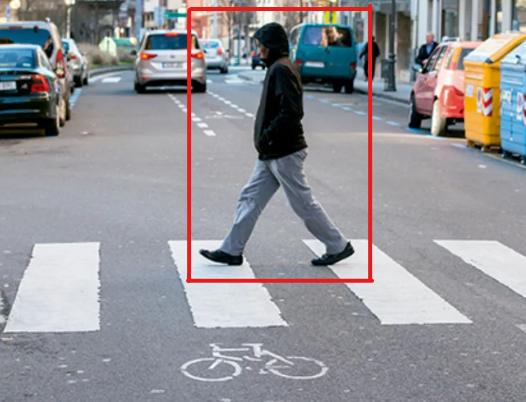
\includegraphics[width=\textwidth]{Figures/2. Related Work/person_detected.png}
        \caption{\textit{
                Person being detected
            }}
    \end{subfigure}
\end{figure}

\begin{equation}
    \left\{
    \begin{array}{ll}
        P_{c} \\
        B_{x} \\
        B_{y} \\
        B_{w} \\
        B_{h} \\
        C_{1} \\
        C_{2} \\
    \end{array}
    \right\}
    \left\{
    \begin{array}{ll}
        1  \\
        50 \\
        70 \\
        60 \\
        70 \\
        0  \\
        1  \\
    \end{array}
    \right\}
\end{equation}

\( P_{c} = \) If there is a car or a person.\\
\( B_{y} = \) Center of object perimeter \((y)\).\\
\( B_{x} = \) Center of object perimeter \((x)\).\\
\( B_{w} = \) perimeter width.\\
\( B_{h} = \) perimeter height.\\
\( C_{1} = \) If there is a car.\\
\( C_{2} = \) If there is a person.\\

But this vector would only represent a correct detection vector of a person in
an image with a region to predict. The previous problem is simplified because
there is still the part in which the image is analyzed to detect the possible
perimeters of objects to pass to the predictor and make its evaluation according
to its training.

In the previous exercise, it gives us an idea of what happens internally, the
convolutional network receives an image with vectors to be evaluated and gives
a prediction based on the analysis and what has been learned. Also the values of
the vectors are assigned according to the prediction and training of the
convolutional network. These vectors have to be organized in a specific way,
have a specific structure, and are analyzed differently depending on the
technique or approach we use to approach this problem.

So far we have seen some parts of the prediction process in images with
convolutional networks, recapitulating:

\begin{itemize}
    \item \textbf{Training of the convolutional network:} moment in which our
          network is going to be trained to classify specific objects, where it is
          going to define the parameters to decide if an object is one thing or
          another.
    \item \textbf{Boundary box detection:} moment in which our program will
          discard and detect the best positioned boundary boxes, which we will predict
          according to the training of the convolutional network.
    \item \textbf{Prediction of elements in the boundary boxes:} the boundary
          boxes found are analyzed and evaluated to find similarity between the
          elements known by the network.
\end{itemize}

\subsection{YOLO (You Only Look Once)}
You Only Look Once (YOLO) is a modern object detection algorithm developed and
published in 2015 by Redmon et al. \cite{yolo_1}. The name of the algorithm is
motivated by the fact that the algorithm only looks once at the image and
requires only one forward propagation pass through the neural network to make
predictions unlike other state of the art object detection algorithms which
work with region proposals and look at the image multiple times. YOLO uses a
single end-to-end convolutional neural network which processes RGB images of
size 448 x 448 and outputs the bounding box predictions for the given image:

\begin{figure}[H]
    \centering
    \begin{subfigure}[b]{0.8\textwidth}
        \centering
        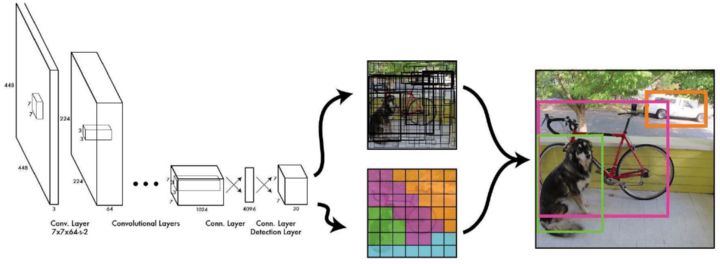
\includegraphics[width=\textwidth]{Figures/2. Related Work/yolo_1.png}
        \caption{\textit{Whole pipeline of YOLO's algorithm} \cite{yolo_images}}
    \end{subfigure}
\end{figure}

It basically reframes object detection as a single regression problem, straight
from image pixels to bounding box coordinates and class probabilities
\cite{yolo_2}. The algorithm divides the input image into an $S x S$ grid
(in the paper $S = 7$). For each grid cell it predicts B bounding boxes
(in the paper $B = 2$), where each bounding box consists of 4 coordinates and a
confidence score for the prediction, and C class probabilities per grid cell
taking the highest one as the final class. All of these predictions are encoded
as an $S x S x (B * 5 + C)$ tensor which is being outputted by the neural
network, as we can see in the following image.

\begin{figure}[H]
    \centering
    \begin{subfigure}[b]{0.6\textwidth}
        \centering
        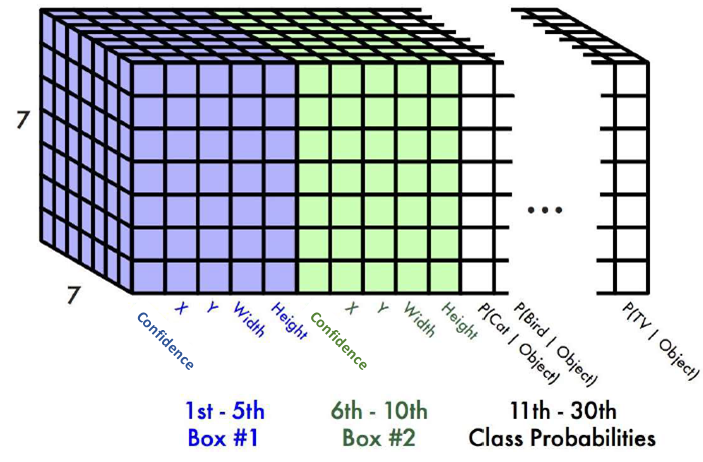
\includegraphics[width=\textwidth]{Figures/2. Related Work/yolo_2.png}
        \caption{\textit{The output tensor of YOLO} \cite{yolo_images}}
    \end{subfigure}
\end{figure}

What the algorithm finally does, is identifying objects in the image and mapping
them to the grid cell containing the center of the object. This grid cell will
be responsible for predicting the final bounding box of the object and will have
the highest confidence score.
In the example of the previous image, each cell of the $7 x 7$ grid is
represented by a vector of size 30 representing a particular area of the image.
Each vector contains 2 bounding box predictions (5 values each) and 20
conditional class probabilities $P(class|object)$. The first step upon extracting
a valid prediction is to choose the bounding box with the higher confidence
score and check if the confidence score is above a predefined threshold
($threshold = 0.25$ in the paper) to output it as a valid prediction. This
confidence score represents the prior in the conditional probability for the
class prediction stating the probability that the given grid cell is the center
of an object with a correct bounding box. To extract the class prediction YOLO
outputs the conditional probability with the highest score. YOLO spatially
defines each bounding box by four coordinates ($X, Y, Width, Height$), where
$(X, Y)$ represent the center of the bounding box relative to the cell, while
$(Width, Height)$ represent the width and the height of the bounding box
relative to the whole image. Because of this, a bounding box can be bigger than
the cell where it was predicted. The cell is only used as the anchor point for
the prediction. One disadvantage of this approach is the fact that every cell
is able to predict only one object. If multiple objects are having their center
points in the same cell, only one will be predicted.

\begin{figure}[H]
    \centering
    \begin{subfigure}[b]{0.6\textwidth}
        \centering
        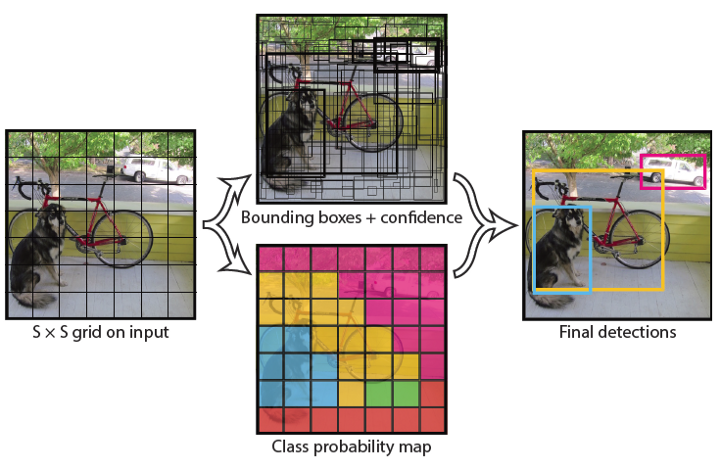
\includegraphics[width=\textwidth]{Figures/2. Related Work/yolo_3.png}
        \caption{\textit{$SxS$ grid and final detections} \cite{yolo_images}}
    \end{subfigure}
\end{figure}

\subsubsection{Model Architecture}
The model architecture consists of 24 convolutional layers followed by 4 pooling layers and 2
fully connected layers.

\begin{figure}[H]
    \centering
    \begin{subfigure}[b]{0.8\textwidth}
        \centering
        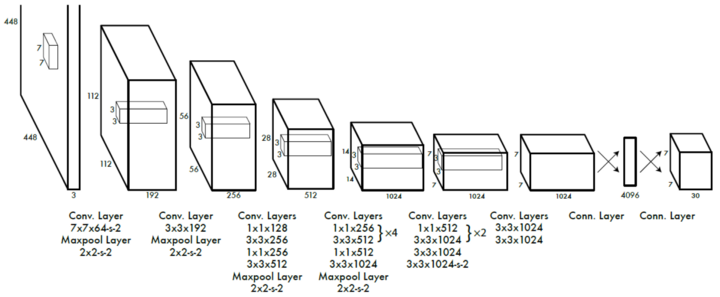
\includegraphics[width=\textwidth]{Figures/2. Related Work/yolo_4.png}
        \caption{\textit{YOLO's model architecture} \cite{yolo_images}}
    \end{subfigure}
\end{figure}

It uses $1 x 1$ convolutions to reduce the amount of feature maps which is
motivated by the Inception Modules of \textit{GoogLeNet} \cite{yolo_3}.
Furthermore it applies the Leaky ReLu activation function after all layers
except for the last one and uses dropout between the two fully connected layers
in order to tackle overfitting.

\subsubsection{Loss Function}
The YOLO algorithm uses a custom loss function in order to control the different
output domains and their influence on the final loss by using special
hyperparameters:

\begin{figure}[H]
    \centering
    \begin{subfigure}[b]{0.8\textwidth}
        \centering
        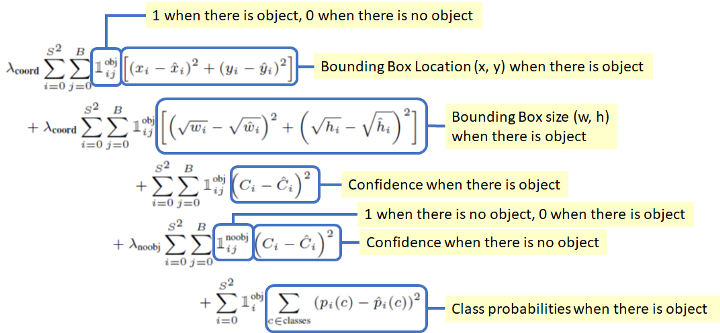
\includegraphics[width=\textwidth]{Figures/2. Related Work/yolo_5.png}
        \caption{\textit{YOLO's custom loss function for every grid cell} \cite{yolo_images}}
    \end{subfigure}
\end{figure}

\begin{enumerate}
    \item \textbf{First term:} penalizes bad locations for the center
          coordinates if the cell contains an object.
    \item \textbf{Second term:} penalizes bad bounding box width and height
          values. The square root is present so that errors in small bounding boxes
          are more penalizing than errors in big bounding boxes.
    \item \textbf{Third term:} penalizes small confidence scores for cells
          containing an object.
    \item \textbf{Fourth term:} penalizes big confidence scores for cells
          containing no object.
    \item \textbf{Fifth term:} simple squared classification loss.
\end{enumerate}

\subsection{SSD (Single-Shot Detector)}
SSD has two components: a backbone model and SSD head. Backbone model usually
is a pre-trained image classification network as a feature extractor. This is
typically a network like ResNet trained on ImageNet from which the final fully
connected classification layer has been removed. We are thus left with a deep
neural network that is able to extract semantic meaning from the input image
while preserving the spatial structure of the image albeit at a lower resolution.
For ResNet34, the backbone results in a $256 7x7$ feature maps for an input
image. We will explain what feature and feature map are later on. The SSD head
is just one or more convolutional layers added to this backbone and the outputs
are interpreted as the bounding boxes and classes of objects in the spatial
location of the final layers activations \cite{ssd_1}.

In the following image, the first few layers (white boxes) are the backbone,
the last few layers (blue boxes) represent the SSD head.

\begin{figure}[H]
    \centering
    \begin{subfigure}[b]{0.8\textwidth}
        \centering
        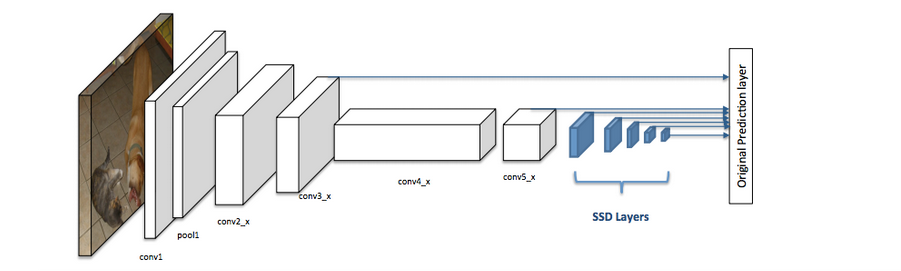
\includegraphics[width=\textwidth]{Figures/2. Related Work/ssd_1.png}
        \caption{\textit{
                Architecture of a convolutional neural network with a SSD detector
            } \cite{ssd_image}}
    \end{subfigure}
\end{figure}

Next, let's go through the important concepts/parameters in SSD, such as
\textit{Grid cell, Anchor box, Aspect ratio, Zoom level and Receptive Field}.

\subsubsection{Grid Cell}
Instead of using sliding window, SSD divides the image using a grid and have
each grid cell be responsible for detecting objects in that region of the image.
Detection objects simply means predicting the class and location of an object
within that region. If no object is present, we consider it as the background
class and the location is ignored. For instance, we could use a 4x4 grid in the
example below. Each grid cell is able to output the position and shape of the
object it contains.

\begin{figure}[H]
    \centering
    \begin{subfigure}[b]{0.5\textwidth}
        \centering
        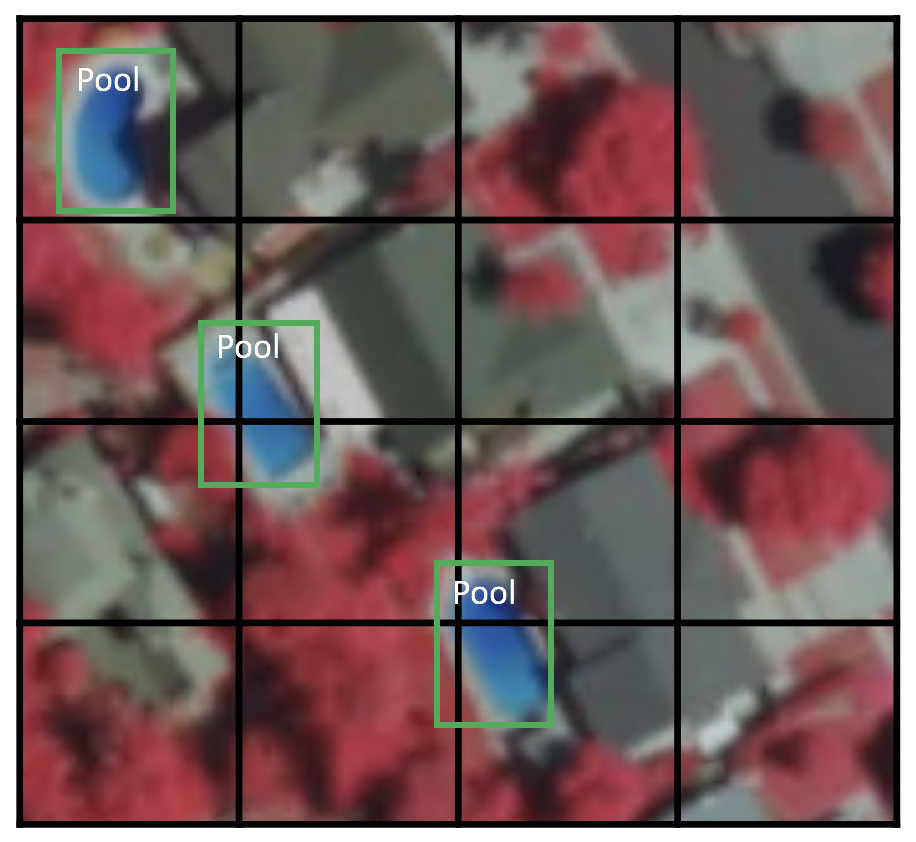
\includegraphics[width=\textwidth]{Figures/2. Related Work/ssd_2.png}
        \caption{\textit{
                Example of a 4x4 grid
            } \cite{ssd_1}}
    \end{subfigure}
\end{figure}

\subsubsection{Anchor Box}
What if there are multiple objects in one grid cell or we need to detect
multiple objects of different shapes. There is why we use anchor box and
receptive field.\\

Each grid cell in SSD can be assigned with multiple anchor/prior boxes. These
anchor boxes are pre-defined and each one is responsible for a size and shape
within a grid cell. For example, the swimming pool in the image below
corresponds to the taller anchor box while the building corresponds to the wider
box.

\begin{figure}[H]
    \centering
    \begin{subfigure}[b]{0.5\textwidth}
        \centering
        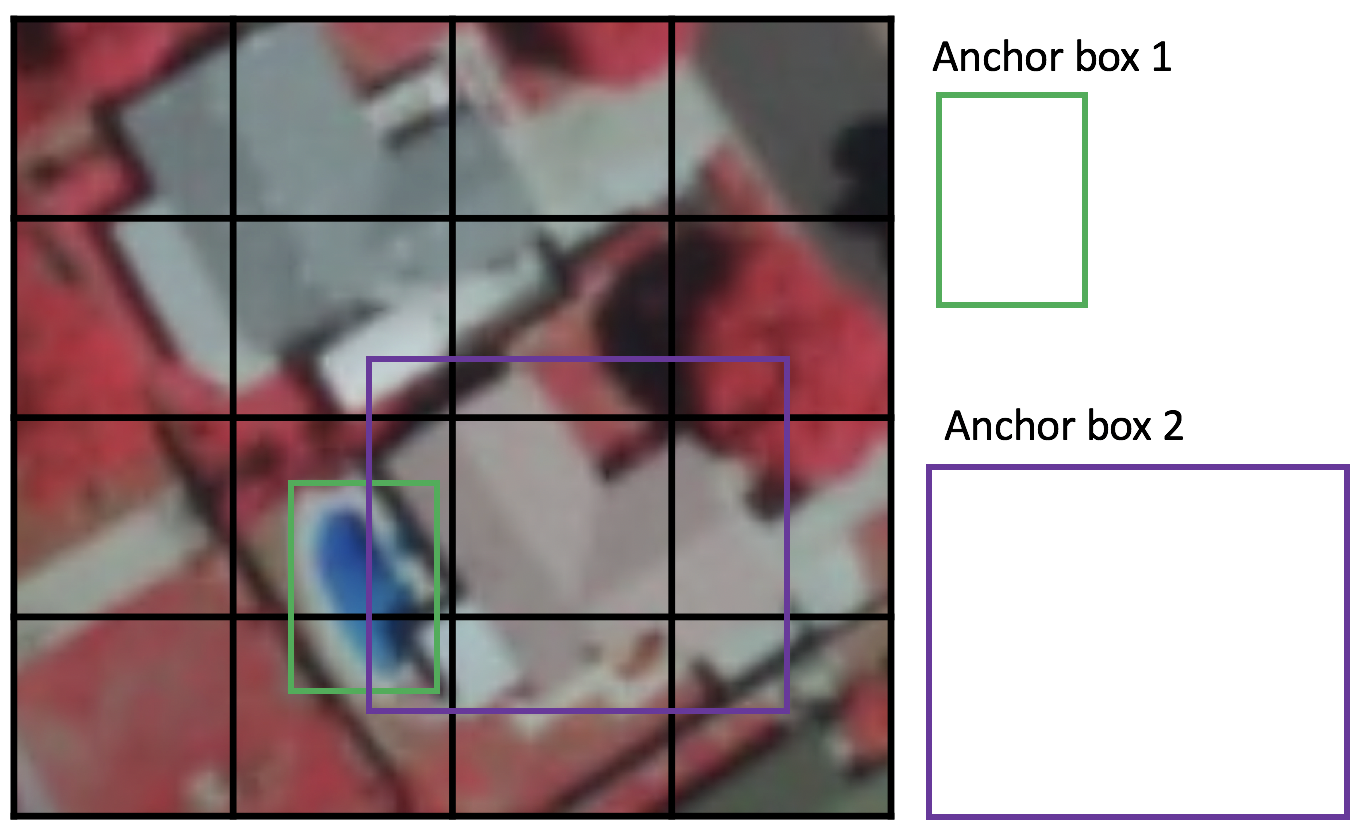
\includegraphics[width=\textwidth]{Figures/2. Related Work/ssd_3.png}
        \caption{\textit{
                Example of two anchor boxes
            } \cite{ssd_1}}
    \end{subfigure}
\end{figure}

SSD uses a matching phase while training, to match the appropriate anchor box
with the bounding boxes of each ground truth object within an image.
Essentially, the anchor box with the highest degree of overlap with an object is
responsible for predicting that object's class and its location. This property
is used for training the network and for predicting the detected objects and
their locations once the network has been trained. In practice, each anchor box
is specified by an aspect ratio and a zoom level.

\subsubsection{Aspect Ratio}
Not all objects are square in shape. Some are longer and some are wider,
by varying degrees. The SSD architecture allows pre-defined aspect ratios of
the anchor boxes to account for this. The ratios parameter can be used to
specify the different aspect ratios of the anchor boxes associates with each
grid cell at each zoom/scale level.

\begin{figure}[H]
    \centering
    \begin{subfigure}[b]{0.5\textwidth}
        \centering
        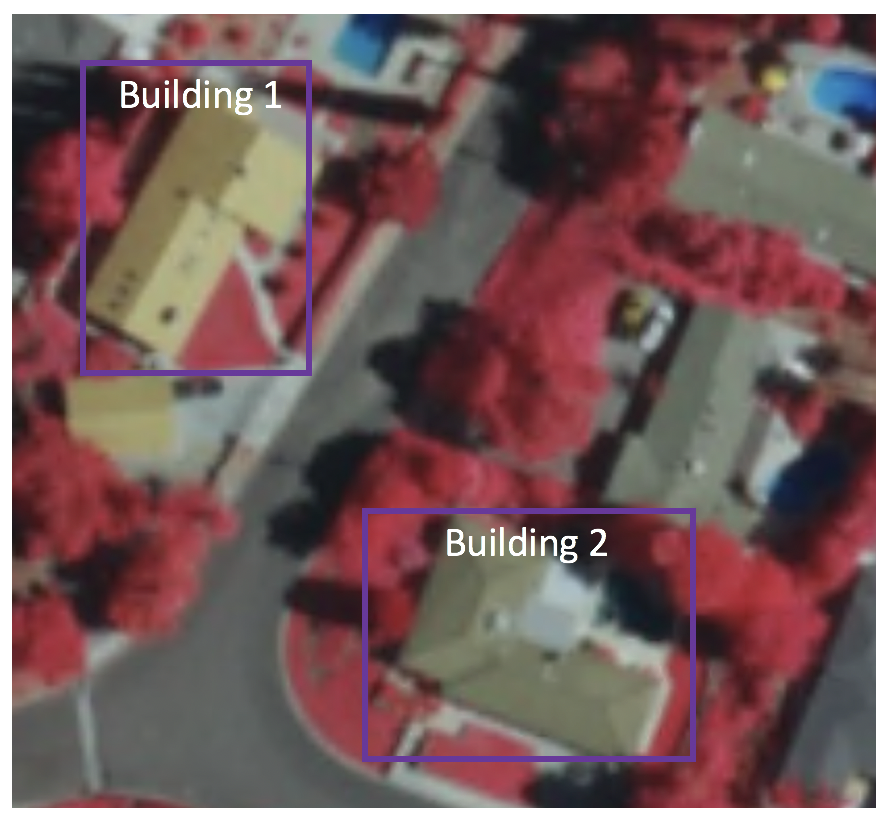
\includegraphics[width=\textwidth]{Figures/2. Related Work/ssd_4.png}
        \caption{\textit{
                The bounding box of building 1 is higher, while the bouding box
                for building 2 is wider
            } \cite{ssd_1}}
    \end{subfigure}
\end{figure}

\subsubsection{Zoom level}
It is not necessary for the anchor boxes to have the same size as the grid cell.
We might be interested in finding smaller or larger objects within a grid cell.
The zooms parameter is used to specify how much the anchor boxes need to be
scaled up or down with respect to each grid cell. Just like what we have seen in
the anchor box example, the size of building is generally larger than swimming
pool.

\subsubsection{Receptive Field}
Receptive field is defined as the region in the input space that a particular
CNN's feature is looking at (also known as "be affected by"). We will use
"feature" and "activation" interchangeably here and treat them as the linear
combination (sometimes applying an activation function after that to increase
non-linearity) of the previous layer at the corresponding location \cite{ssd_2}.
Because of the the convolution operation, features at different layers represent
different sizes of region in the input image. As it goes deeper, the size
represented by a feature gets larger. In this example below, we start with the
bottom layer $(5x5)$ and then apply a convolution that results in the middle layer
$(3x3)$ where one feature (green pixel) represents a $3x3$ region of the input
layer (bottom layer). And then apply the convolution to middle layer and get the
top layer $(2x2)$ where each feature corresponds to a $7x7$ region on the input
image. These kind of green and orange 2D array are also called feature maps
which refer to a set of features created by applying the same feature extractor
at different locations of the input map in a sliding window fastion. Features
in the same feature map have the same receptive field and look for the same
pattern but at different locations. This creates the spatial invariance of ConvNet.

\begin{figure}[H]
    \centering
    \begin{subfigure}[b]{0.8\textwidth}
        \centering
        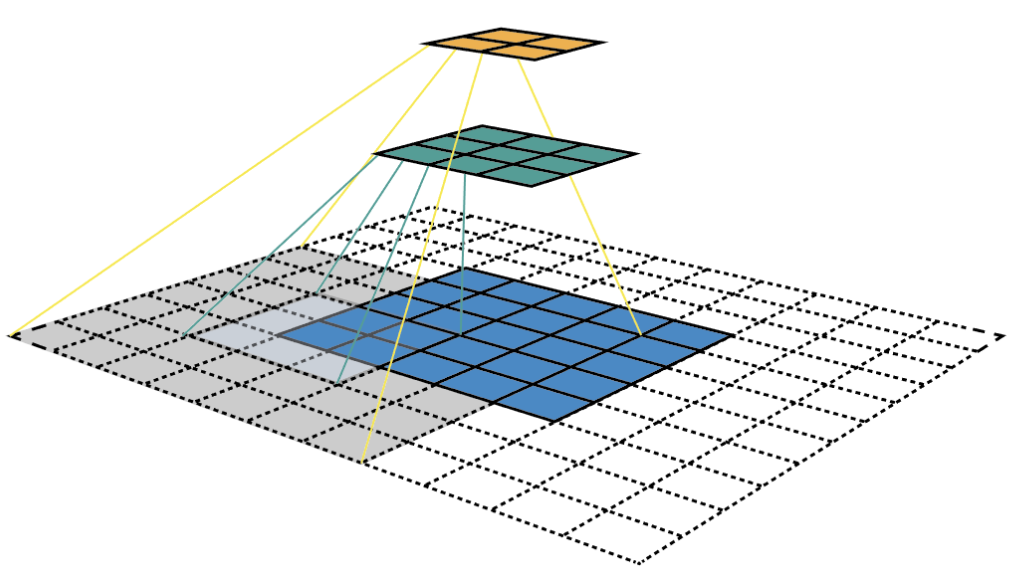
\includegraphics[width=\textwidth]{Figures/2. Related Work/ssd_5.png}
        \caption{\textit{
                Visualizing CNN feature maps and receptive field
            } \cite{ssd_1}}
    \end{subfigure}
\end{figure}

Receptive field is the central premise of the SSD architecture as it enables us
to detect objects at different scales and output a tighter bounding box. Why? As
you might still remember, the ResNet34 backbone outputs a $256 7x7$ feature maps
for an input image. If we specify a 4x4 grid, the simplest approach is just to
apply a convolution to this feature map and convert it to $4x4$. This approach can
actually work to some extent and is exatcly the idea of YOLO.
The extra step taken by SSD is that it applies more convolutional layers to the
backbone feature map and has each of these convolution layers output a object
detection results. As earlier layers bearing smaller receptive field can
represent smaller sized objects, predictions from earlier layers help in dealing
with smaller sized objects.

Because of this, SSD allows us to define a hierarchy of grid cells at different
layers. For example, we could use a $4x4$ grid to find smaller objects, a $2x2$ grid
to find mid sized objects and a $1x1$ grid to find objects that cover the entire
image.

\subsection{R-CNN (Region-Based Convolutional Networks)}
Generally, these object detection and deep learning algorithms focus on solving
problems or problems that arise when assigning the task to a machine to detect
things; the training time of the convolutional network, the operations necessary
for the input element, among many other things that are summarized to reduce
complexity and guarantee a correct prediction. In the case of RCNN, it proposes
a solution based on an initial segmentation from predefined mathematical models
to give property to the objects to be predicted \cite{rcnn_1}, from there it is
segmented into regions that with each iteration can become more detailed or more
imprecise, depending on the defined properties, the image, the training time,
etc.\\

The RCNN algorithm is intended to improve the boundary box selection process in
an image, where with each iteration, it generates more general boundary boxes,
but much faster. It works in such a way that it proposes regions to an input
image based on a segmentation process. This segmentation process ensures having
regions that really have objects to classify by proposing a process in which,
instead of going through the entire image trying to detect whether there is an
object or not, it creates regions (as we will see in the next picture) from the
properties of the pixels in the image. Those with hue, light, texture and any
attribute to take into account, are grouped into regions by proximity,
generating a first iteration of the image in which the regions with the most
similar colors of the image are obtained. Each region has a weight or value that
makes it similar to nearby regions (in the case of the figure it would be the
color assigned to the region based on the properties).

\begin{figure}[H]
    \centering
    \begin{subfigure}[b]{0.8\textwidth}
        \centering
        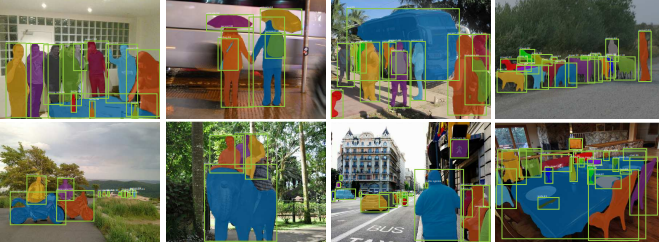
\includegraphics[width=\textwidth]{Figures/2. Related Work/rcnn_1.png}
        \caption{\textit{He, K. Gkioxari, G. Dollar, P. Girshick, R. Mask R-CNN.
                \url{https://openaccess.thecvf.com/content_ICCV_2017/papers}
            }}
    \end{subfigure}
\end{figure}

When the image has gone through several iterations in which the regions are
mixed with other neighboring regions that have a (statistical) resemblance,
the machine is capable of generating prediction zones of interest, minimizing
the possible object perimeters to be evaluated, making easier the
differentiation of objects and reducing the complexity of the input \cite{rcnn_1}.

How this method differs from a normal CNN is that the input image went through
a region segmentation and classification process for faster filtering and
analysis.

\begin{figure}[H]
    \centering
    \begin{subfigure}[b]{0.6\textwidth}
        \centering
        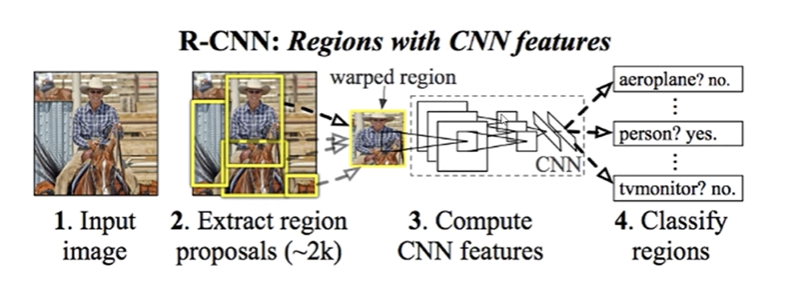
\includegraphics[width=\textwidth]{Figures/2. Related Work/rcnn_2.png}
        \caption{\textit{'Sliding Windows' Algorithm Taken from:
                \url{https://www.youtube.com/watch?v=vr5rs_cTKCs&t=136s&ab_channel=DeepLearning}
            }}
    \end{subfigure}
\end{figure}

\subsection{Fast R-CNN and Faster R-CNN}
Basically, convolutional network implementations for object detection always
seek, optimization of resources, time, and accuracy. Over the years researchers
realized that finding the regions for the perimeter boxes could be slow and
clunky and devised a way to make this process faster. They found a way to
implement the 'Sliding Windows' technique to obtain the object perimeter boxes
efficiently, using convolutional networks (CNN).\\

The fast R-CNN uses RoI (regions of interest) which it converts into feature
maps. In this way, it reduces the image vector to a smaller feature map and is
able to use it when deciding on a prediction \cite{rcnn_2}.\\

Siliding Windows: In object detection problems, we generally have to find all
possible objects in the image, such as all cars in the image, all pedestrians
in the image, all bicycles in the image, etc. To do this, we use an algorithm
known as sliding window detection. Let's understand this algorithm.

\begin{itemize}
    \item In this algorithm (Sliding Windows), we choose a grid cell of a
          specific size (Let's choose a $2x2$).
    \item We overlay the previous grid cell across the image and convolve the
          part of the image in the grid cell and predict the output.
    \item We then overlay the grid cell via a second jump and then convolve the
          next part of the image.
\end{itemize}

Thus, we cover the entire image. We repeat the same procedure with different
sizes of grid cells.

\begin{figure}[H]
    \centering
    \begin{subfigure}[b]{0.8\textwidth}
        \centering
        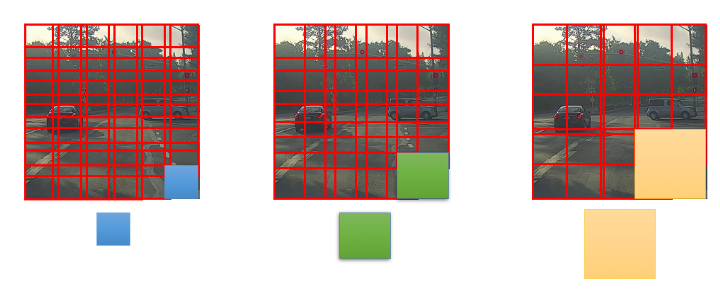
\includegraphics[width=\textwidth]{Figures/2. Related Work/rcnn_3.png}
        \caption{\textit{'Sliding Windows' Algorithm Taken from:
                \url{https://medium.com/ai-quest/convolutional-implementation-of-the-sliding-window-algorithm-db93a49f99a0}
            }}
    \end{subfigure}
\end{figure}

This approach has advantages and disadvantages. where we can find:
\begin{itemize}
    \item It is time consuming by the number of times the image iterates to get
          predictions.
    \item Consumes a good amount of resources.
    \item It is slightly less accurate (on perimeter boxes).
    \item Quickly discard unnecessary predictions.
\end{itemize}

Going back to fast R-CNN, this implementation makes a Windows slinding approach
to generate predictions of the regions to be analyzed, reducing the vectors
(that is, they go through a transformation process according to the regions of
interest, converting them into small feature maps, reducing the problem). \cite{rcnn_2}

\begin{figure}[H]
    \centering
    \begin{subfigure}[b]{0.8\textwidth}
        \centering
        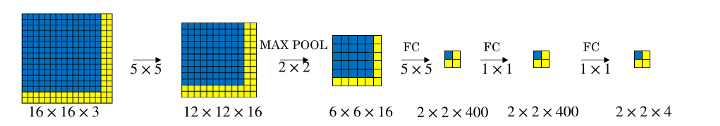
\includegraphics[width=\textwidth]{Figures/2. Related Work/rcnn_4.png}
        \caption{\textit{'Sliding Windows' Algorithm Taken from:
                \url{https://medium.com/ai-quest/convolutional-implementation-of-the-sliding-window-algorithm-db93a49f99a0}
            }}
    \end{subfigure}
\end{figure}

By reducing the vectors trying to predict the objects we generate a smaller
data collection. Also, by implementing the sliding window in the image (because
each object to classify would have a possible sliding window, represented in a
minimized vector). I must also say that one of the features of fast R-CNN to
make it optimal is to run the sliding Windows algorithm ONLY ONE time, this way
it is faster, although slightly less accurate. Making it better for detecting
large objects.